\documentclass[conference]{IEEEtran}
\usepackage[dvips]{graphicx}
\usepackage{latexsym}
\usepackage{subfig}
%\usepackage{float}
\usepackage{url}
%\usepackage{amsmath}

%\usepackage{ifpdf}
%\usepackage{cite}
\ifCLASSINFOpdf
  % \usepackage[pdftex]{graphicx}
  % declare the path(s) where your graphic files are
  % \graphicspath{{../pdf/}{../jpeg/}}
  % and their extensions so you won't have to specify these with
  % every instance of \includegraphics
  % \DeclareGraphicsExtensions{.pdf,.jpeg,.png}
\else
  % or other class option (dvipsone, dvipdf, if not using dvips). graphicx
  % will default to the driver specified in the system graphics.cfg if no
  % driver is specified.
  % \usepackage[dvips]{graphicx}
  % declare the path(s) where your graphic files are
  % \graphicspath{{../eps/}}
  % and their extensions so you won't have to specify these with
  % every instance of \includegraphics
  % \DeclareGraphicsExtensions{.eps}
\fi
\usepackage[cmex10]{amsmath}
%\usepackage{algorithmic}
%\usepackage{array}
%\usepackage{mdwmath}
%\usepackage{mdwtab}
%\usepackage{eqparbox}
%\usepackage[tight,footnotesize]{subfigure}
%\usepackage[caption=false]{caption}
%\usepackage[font=footnotesize]{subfig}
%\usepackage[caption=false,font=footnotesize]{subfig}
%\usepackage{fixltx2e}
%\usepackage{stfloats}
%\usepackage{url}
% correct bad hyphenation here
%\hyphenation{op-tical net-works semi-conduc-tor}

\begin{document}
\title{Relaxing CDN energy}

% author names and affiliations
% use a multiple column layout for up to three different
% affiliations


%\author{\IEEEauthorblockN{Michael Shell\IEEEauthorrefmark{1},
%Homer Simpson\IEEEauthorrefmark{2},
%James Kirk\IEEEauthorrefmark{3}, 
%Montgomery Scott\IEEEauthorrefmark{3} and
%Eldon Tyrell\IEEEauthorrefmark{4}}
%\IEEEauthorblockA{\IEEEauthorrefmark{1}School of Electrical and Computer Engineering\\
%Georgia Institute of Technology,
%Atlanta, Georgia 30332--0250\\ Email: see http://www.michaelshell.org/contact.html}
%\IEEEauthorblockA{\IEEEauthorrefmark{2}Twentieth Century Fox, Springfield, USA\\
%Email: homer@thesimpsons.com}
%\IEEEauthorblockA{\IEEEauthorrefmark{3}Starfleet Academy, San Francisco, California 96678-2391\\
%Telephone: (800) 555--1212, Fax: (888) 555--1212}
%\IEEEauthorblockA{\IEEEauthorrefmark{4}Tyrell Inc., 123 Replicant Street, Los Angeles, California 90210--4321}}


\author{\IEEEauthorblockN{Mohamad Dikshie Fauzie\IEEEauthorrefmark{1} \quad
Achmad Husni Thamrin\IEEEauthorrefmark{1} \quad
Rodney Van Meter\IEEEauthorrefmark{2} \quad
Jun Murai\IEEEauthorrefmark{2}}
\IEEEauthorblockA{\IEEEauthorrefmark{1}Graduate School of Media and Governance} \quad
\IEEEauthorblockA{\IEEEauthorrefmark{2}Faculty of Environment and Information Studies\\ 
Keio University, 252-0882 Kanagawa, Japan \\
dikshie@sfc.wide.ad.jp \quad\quad husni@ai3.net \quad\quad rdv@sfc.wide.ad.jp \quad\quad jun@wide.ad.jp}
}
% make the title area
\maketitle
\IEEEpeerreviewmaketitle

\begin{abstract}

Many CDN companies utilize peer-to-peer to scaling the services and saving bandwidth.
However, we still have little knowledge about the energy consumption in peer-assisted CDN.
This paper presents an analysis of a energy consumption in peer-assisted CDN system, where an ISP manages its own CDN and its users participate in a P2P network to assist content delivery.
To evaluate energy consumption in peer-assisted CDN, we take two cases: (1) live stream and (2) online storage.
We developed a simple energy consumption model for live streaming service and online storage service and evaluate this model using a empirical existing live streaming model and online storage model.
We find that in live streaming service, total energy system increase with growing number of peers.
However, if we concern only on CDN service part, delegate part of workload to peers can save CDN server up to $11\%$ compare to pure CDN architecture, while total energy system difference with pure CDN only less than $1\%$. 
In peer assisted online storage, we study three server bandwidth allocation strategies: (1) theoretical lower bound, (2) request driven, and (3) water level.  
total energy system depends on strategies of server bandwidth allocation.
Compare to pure CDN architecture peer-assisted, peer assisted online storage total system energy saving less than $1\%$.
\end{abstract}


%\begin{keyword}
%CDN, Data Center, Energy, Peer Assisted, P2P
%\end{keyword}

\maketitle

%1
\section{Introduction}\label{intro}
Streaming content, especially video, represents a significant fraction of the traffic volume on the Internet, and it has become a standard practice to deliver this type of content using Content Delivery Networks (CDNs) such as Akamai and Limelight for better scaling and quality of experience for the end users.  
For example, Youtube uses Google cache and MTV uses Akamai in their operations.

With the spread of broadband Internet access at a reasonable flat monthly rate, users are connected to the Internet 24 hours a day and they can download and share multimedia content.  
P2P (peer to peer) applications are also widely deployed.  
In China, P2P is very popular; we see many P2P applications from China such as PPLive, PPStream, UUSe, Xunlei, etc.  
Some news broadcasters also rely on P2P technology to deliver popular live events.  
For example, CNN uses the Octoshape solution that enables their broadcast to scale and offer good video quality as the number of users increases.

From the Internet provider point of view, the presence of so many always-on users suggests that it is possible to delegate a portion of computing, storage and networking tasks to the users, thus creating P2P networks where users can share files and multimedia content.
Starting from file sharing protocols, P2P architectures have evolved toward video on demand and support for live events.

Broadband network access helps P2P applications to perform better.
xDSL networks are deployed worldwide, and in some countries, such as Japan, even higher bandwidth fiber to the home (FTTH) already exceeds DSL in market penetration.  In the coming years, FTTH will be massively deployed by network operators throughout the world.  
As access bandwidth increases, P2P systems may become more efficient since a peer can contribute much more.

In Peer assisted CDN \footnote{in this paper, we may interchange peer assisted CDN and CDN-P2P.}, users can download content from CDN nodes for from other users or peers the content.
A user may cache the content after download to serve requests from other users
Due to complexity of behavior of peers, the process should be done in home gateway user where ISP can have control on it. 

On the other hand, data center where CDN server placed faces costs for powering the data center.
The Uptime Institute, a global data center authority, surveyed 1100 data center owners and operators on 2012, reported that 55\% organizations must increase budget 10\% than 2011 \cite{uptime}.  
30\% of organizations will run out of data center capacity (power, cooling, space, and network) in the end of 2012 \cite{uptime}. 
More than 50\% organizations surveyed reported that saving energy \footnote{in this paper, we may interchange energy and power.} is major priority \cite{uptime}.
Even in the data centers using the state of art cooling technologies heat dissipation accounts for at least $20\%$ until $50\%$ of the total power consumption 
\cite{google}.
The increases in energy cost and the demand due to growth of traffic urges the data center operators and owners to look for ways to reduce energy usage in the years to come.
Although reducing energy consumption can effectively reduce overall cost, this will limit the capacity growth and scalability of the service provisioning.
For example: routers and servers spend most of their energy on the baseline activities such as running the fans, spinning hardisks, powering backplane, and powering the memory. 
Even in an idle state, modern systems can be consuming anything from $50\%$ until $80\%$ of the power consumed under maximum load \cite{4404806,4509688}.
Alternatively, the data center and be revamped by relocating some services to end-host computers or peers.
Peers contribute their communication, storage, and computation resources to exchange data and provide services while the data center performs central administration and authentication as well as backend processing.
P2P network, formed by peers offer flexibility and scalability in service delivery.
%Therefore, P2P services can assist and enhance data center.
It is not our aim to advocate one system architecture over another.
Many issue such as manageability, reliability, and ease of deployment must be taken into account when making high level architectural decisions.

In this paper, we study the energy consumption of hybrid CDN-P2P.  
It has been known that CDN energy consumption is better than P2P architecture \cite{feldmann2010energy,baliga2007energy}, unfortunately that model only think small part of problem energy consumption (devices/hardwares).
To be fair, we also need to see how combination of some architectures can help to reduce energy footprint, for example: combination of CDN and P2P.
%If we can move part of computation resource from CDN in data center to P2P, then we can relax power budget of data center for hardware and cooling. 

The rest of this paper is organized as follows. 
Section 2 present motivation of this paper.
Section 3 provides an overview of system model, data center model and energy model.  
In section 3, we will present result and analysis.  
Section 4 will conclude this paper. 

\begin{figure}[tb]
\begin{center}
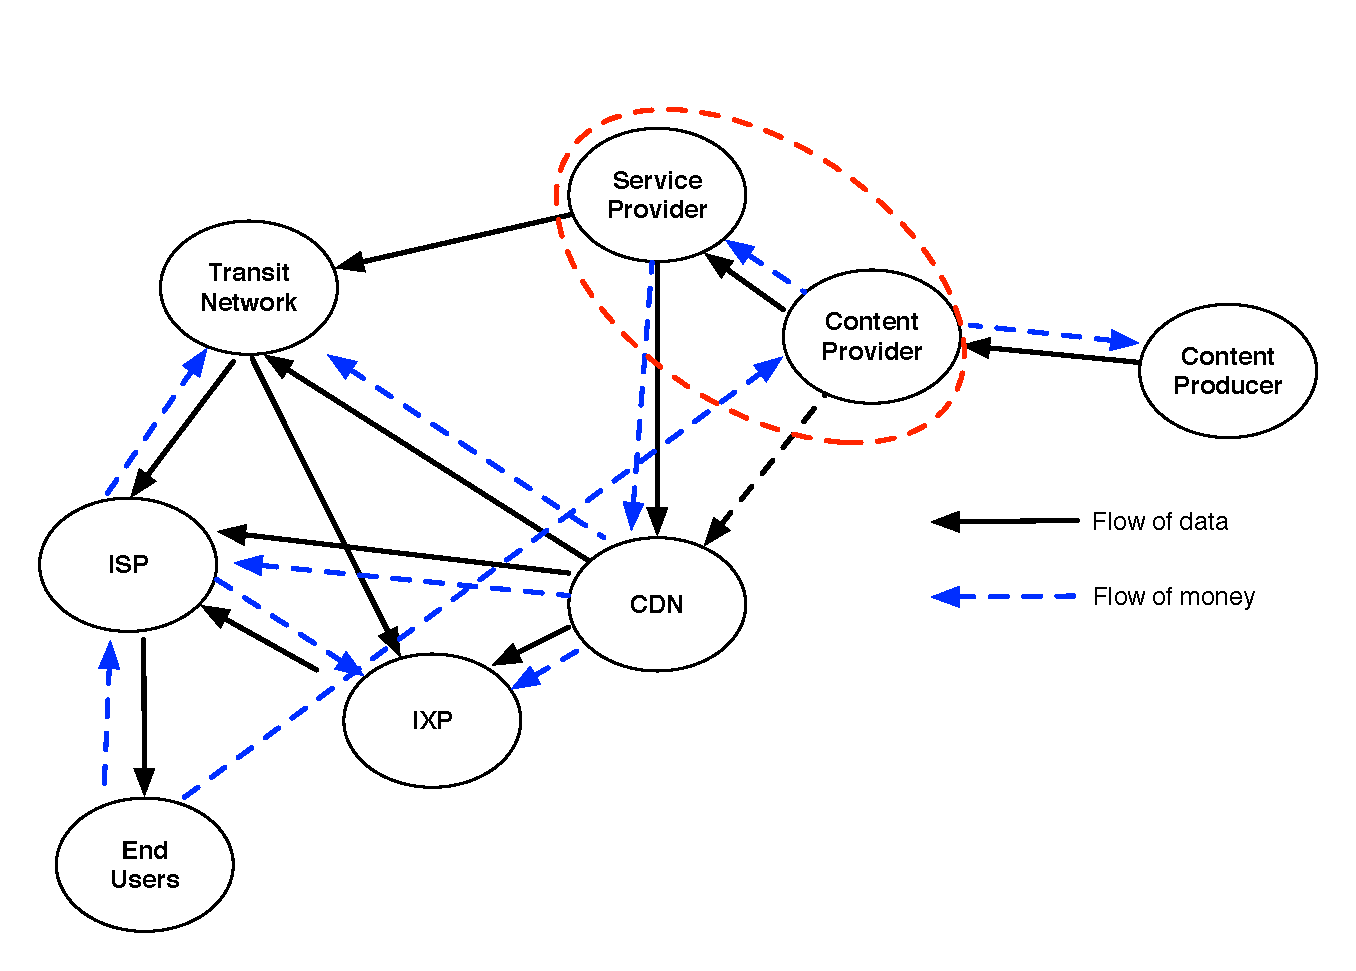
\includegraphics[scale=0.4]{graphs/business-relationship.eps}
\end{center}
\caption{In Complex relationship of entities in Internet, 
CDN mostly placed in data center near to eyeball ISP. 
If CDN can not reach eyeball ISP due to business or economic reason, CDN can be placed near to IXP or even inside IXP, and CDN will reach eyeball ISP from peering point inside IXP.}
\label{fig:businessrelationship}
%\vspace{-2mm}
\end{figure} 

\section{Motivation}\label{motivation}
In the economic supply chain of video traffic, most ISPs get a little revenue from video traffic thus ISP wants to monetize that traffic.
the future of CDN business is likely to live deeper into ISP networks, more integrated into and interleaved with ISP infrastructures thus users can get good quality of video.
The idea of ISP managed CDN has been proposed in recent years.
The complexity of the CDN business encourage ISP to manage their own CDN rather than allow others to run CDNs on their networks.

CDN architectures are host-oriented: content is delivered to end users through host servers that are centrally managed in a few data centers fig.\ref{fig:businessrelationship}. 
The growing of Internet traffic dominated by video, the energy consumption of a host oriented architecture becomes problematic due to over provisioning factor.
The idea of utilizing the user's computation power to support ISP operation is not new. 
The figaro project proposed residential gateway as an integrator of different networks and services, becoming an Internet wide distributed content management for a proposed future Internet architecture.  
The important key in this architecture is both user home gateway and access bandwidth controlled and managed by ISP.
In this case, ISP can offload part of workload on their CDN to user's home gateway.  
By offloading workload, their CDN can relax energy demand thus relaxing data center power budget or relaxing capacity planning for power.
This architecture depends largely on the number of devices which can be found online at a point in time.
While some users keep their home gateway online at all times, there are small number of users might turn off or their home gateway can not be reached.
Based on study from Dischinger et al., \cite{Dischinger:2007:CRB:1298306.1298313} and Valancius et al., \cite{valancius2009greening}, the average availability of the residential gateways in 12 major ISPs over one month is up $85\%$ with $5\%$ until $8\%$ uptime variations thought out a day.

\section{System Description}\label{system model}
\begin{figure}[thb]
\begin{center}
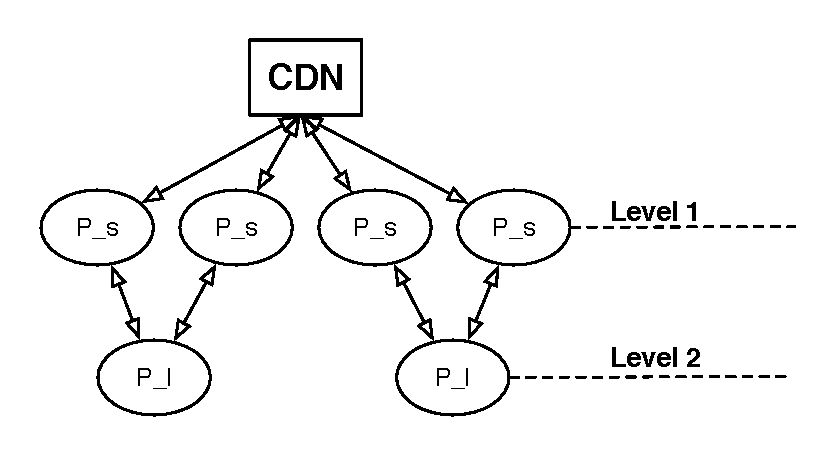
\includegraphics[scale=0.6]{graphs/p2p-cdn.eps}
\end{center}
\caption{Example model of content delivery architecture with peer assisted.}
\label{fig:iptv}
\end{figure} 

Figure \ref{fig:iptv} shows example model of CDN with peer assisted for live streaming \cite{Yin:2010:LEC:1823746.1823750}.  
$P_s$ in fig.\ref{fig:iptv} is peers in level 1 or seeders.  
Seeders get content directly from CDN.  
$P_l$ in fig.\ref{fig:iptv} is peers in level 2 or leechers.
Leechers get content from seeders.

Maximum number of seeders is bounded by maximum CDN's capacity, while maximum number of leechers in level 2 is bounded by number of seeders can support the bitrate.
Denote number of seeders is $n_s$, number of leechers is $n_l$, $\rho$ is maximum bitrate that supplied by seeders to leechers, and $r=1$ is video bitrate, therefore we have number of leechers that can be supported by seeders is:

\begin{equation}\label{eqn:leecher}
	\lfloor n_l \rfloor = n_s . \rho
\end{equation}

Number of seeders that support or upload content to leecher is:

\begin{equation}\label{eqn:seeders-to-leechers}
	n_{s}^{u} = n_l . \frac{r}{\rho}
\end{equation}

The illustration as follows, suppose we have video bitrate $r=1$, seeder upload rate $\rho=0.25$, and maximum CDN capacity is $643Mbps$. 
Maximum number of seeders supported by CDN is $n_s=643$.
Maximum number leechers supported by seeders is $n_l=160$.  
Number of seeders that upload content to leechers is $n_{s}^{u}=640$.  
Therefore we have three seeders that do not need to upload content to leecher. 


\subsection{Abstracting Data Center Power}\label{thermodynamics}
\begin{figure}[thb]
\begin{center}
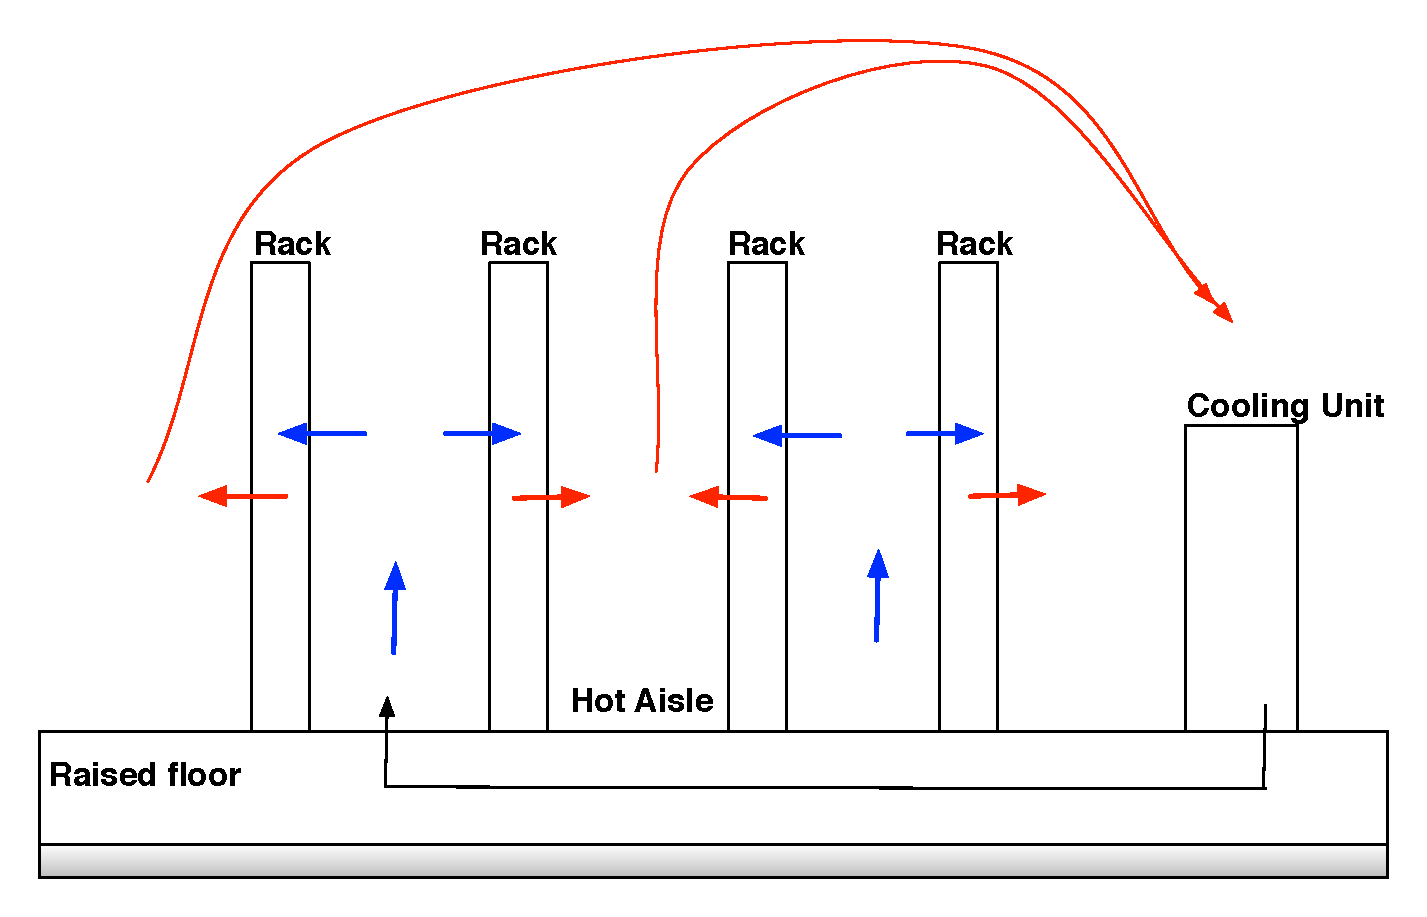
\includegraphics[scale=0.3]{graphs/datacenter.eps}
\end{center}
\caption{A typical data center schematic.
The cooling infrastructure comprises industry standard racks on a raised floor, through which multiple compressor-driven computer room air conditioning unit circulate cool air through a share plenum.}
\label{fig:datacenter}
%\vspace{-2mm}
\end{figure} 
Many aspects involved in power management in data center and interactions among power management strategies across subsystems grow more complex.
Five distinct subsystems account for most of a data center's power draw:   server and storage systems, power conditioning equipment, cooling and humidification systems, networking equipment, and lighting/physical security.
In this section, we only focus on relationship between cooling power and hardware temperature.

Data center seek to provision the cooling adequately to extract the heat produce by servers, switches, routers, and other devices.
Practically, cooling provisioning are done at facilities level.
Data center operator operate cooling facilities based on power ratings of servers, switches, routers, and other devices often with some additional headroom for risk tolerance. 
The compounded over provisioning of computing and cooling infrastructures can drive up initial and recurring costs. 

The cooling cycle of a typical data center operates in the following way:
Cooling units operate by extracting heat from the data center and pumping cold air into the room, usually through a pressurized floor plenum.
The pressure forces the cold air upward through vented tiles, entering the room in front the hardware
Fans draw the cold air inward and through the server; hot air exits through the rear of the server.
The hot air rises sometimes with the aid of fans and a ceiling plenum , and is sucked back to the cooling units.
The cooling units force the hot air past pipes containing cold air or water. 
The heat from the returning air transfer through the pipes to the cold substance. 
The heated substance leaves the room and goes to a chiller and cooling unit fans force the cold air back into the floor plenum. 
Above process is shown in fig.\ref{fig:datacenter}

The efficiency of this cycle depends on several factors, including the conductive substance and the air flow velocity, but it is quantified by coefficient of performance (COP).
The COP is the ratio of heat removed ($Q$) to the amount of work necessary ($W$) to remove that heat:

\begin{equation}\label{eqn:cop}
	COP=\frac{Q}{W}
\end{equation}

Therefore, the work necessary to remove heat is inversely proportional to the COP.  
A higher COP indicates a more efficient process, requiring less work to remove a constant amount of heat.

However, the COP for a cooling cycling is not constant, increasing with the temperature of the air the cooling unit pushes into the plenum.  
COP value empirically can be computed using \cite{moore2005making}:

\begin{equation}\label{eqn:copt}
	COP(T) = 0.0068.T^2 + 0.0008.T + 0.458
\end{equation}

where $T = T_{sup} + T_{adj}$ and $T_{adj} = T_{safe}^{in}-T_{max}^{in}$. \\
$T_{sup}$ is temperature supply by cooling unit and $T_{adj}$ is temperature difference between maximum safe hardware inlet temperature ($T_{safe}^{in}$) and the maximum observed hardware inlet temperature ($T_{max}^{in}$).
If $T_{adj}$ is negative, it indicates that a hardware inlet exceeds maximum safe temperature thus we need to lower $T_{sup}$ to bring the hardwares back below the system temperature level.

\begin{figure}[thb]
\begin{center}
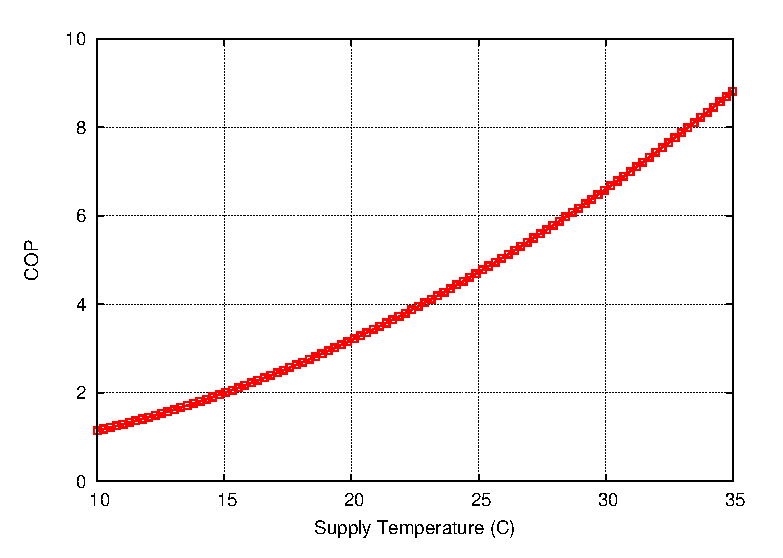
\includegraphics[scale=0.6]{graphs/cop.eps}
\end{center}
\caption{COP curve for the chilled water cooling units from HP Lab utility data center.
As the target temperature of the air the cooling unit pumps into the floor plenum increases, the COP increases.}
\label{fig:twotier}
%\vspace{-2mm}
\end{figure} 

Cooling cost can be calculated as  \cite{moore2005making} :

\begin{equation}\label{eqn:cost}
C = \frac{Q}{COP(T)}
\end{equation}

Where $Q$ is amount of power the servers and hardwares consume.
COP(T) is our COP at $T=T_{sup}+T_{adj}$.
Currently we assume a uniform $T_{sup}$ from each cooling units due to the complications introduced by non-uniform cold air supply.


\subsection{Energy Model}\label{energy model}
In this paper, our goal is to provide a general view and a fair comparison of the energy consume by a CDN and hybrid CDN-P2P architecture. 
To do so, we designed a series of model and perform an analysis.
Our energy model is similar to the models used in \cite{Nedevschi:2008:HDC:1855610.1855618}.
The difference with \cite{Nedevschi:2008:HDC:1855610.1855618}, our baseline energy is not function of bitrate flow. 
Our baseline energy is based on minimum energy required to turn-on the device without any traffic low trough the device. 
Network model for energy is assumed to be flat network as shown in fig.\ref{fig:iptv}.

For each component, we consider two energy measurement:  baseline energy consumption and energy consumed per work unit $\delta$.
The baseline energy is the energy consumed to keep the device on.
Even when there is no traffic, the device still consume energy.
The energy consumption for a single request in CDN server as:
\begin{equation}\label{eqn:E_d}
	E_{d} = E_s
\end{equation}
while the energy consumption for a single request in network as:
\begin{equation}\label{eqn:E_r}
	E_{r} = d_s.E_r
\end{equation}
and energy of peer or client is $E_p$.

where $d_s$ is number of hops or the path length.
We define $\delta_s$ and $\delta_r$ work-induced energy consumed per additional bit transferred by a server and router.   
We can express these per-bit work induced consumptions as follows:
\begin{equation}\label{eqn:delta_s}
	\delta_s = \frac{(S_{max} - S_{base})}{M_s} 
\end{equation}
$S_{base}$ is a server's baseline power consumption.  
$S_{max}$ is a server's power when operating at maximum capacity.
$M_s$ is the maximum capacity in bit per second for a server.
Same formulation also applied for network component.  
\begin{equation}\label{eqn:delta_r}
	\delta_r = \frac{(R_{max} - R_{base})}{M_R} 
\end{equation}
$R_{max}$ is a router power when operating at maximum capacity.
$R_{base}$ is a router's baseline power consumption.
$M_R$ is maximum capacity in bit per second for a router.

Substituting eq.\ref{eqn:delta_s}, and eq.\ref{eqn:delta_r} to eq.\ref{eqn:E_d} and eq.\ref{eqn:E_r}, we can rewrite eq.\ref{eqn:E_d} and eq.\ref{eqn:E_r} as follows:
\begin{equation}\label{eqn:E_d dan E_r}
\begin{split}
	E_{d} &= \delta_s.B + E_{s-baseline}\\
	E_{r} &= d_s.\delta_r.B + E_{r-baseline}\\
	E_{p} &= \delta.B + E_{p-baseline}
\end{split}
\end{equation}
Finaly total energy is:
\begin{equation}\label{eqn:E_t}
\begin{split}
	E_{t} &= E_d + E_r + E_p \\
	E_{t} &= \delta_s.B + E_{s-baseline} + d_s.\delta_r.B + E_{r-baseline} + \delta_p.B + E_{p-baseline}
\end{split}
\end{equation}
where $B$ is size of file to be transferred. 

Considering cooling energy, we can substitute eq.\ref{eqn:cost} to eq.\ref{eqn:E_t}, therefore total energy consumption: 
\begin{equation}
	\hat{E}_{t} = E_{t}.\left( 1+\frac{1}{COP(T)} \right)
\end{equation}

%We also considering content popularity distribution.   
%We assume that content provider has a content catalog of size $F$, ranked from 1 to $F$ based on popularity.   
%$1$ represents the most popular content.
%Letting the total number of requests in a given time duration $t$ will be $R$, the number of requests for content of popularity $k$, $R_k$ follows Zipf distribution as:

%\begin{equation}
%	R_k = R \frac{k^{-\beta}}{\sum_{k=1}^F k^{-\beta}}
%\end{equation}
%A large $\beta$ indicates a relatively small set of very popular content.
%Typical value of $\beta$ range between $0.5$ and $1.0$.
%IPTV channel has $\beta=0.8$ \cite{Cha:2008:NTP:1855641.1855646}.


\section{Result and Discussion}\label{analysis}
\subsection{Live Streaming}
For numerical simulation, we use work induced energy consumed per second from \cite{Nedevschi:2008:HDC:1855610.1855618}.
For CDN server baseline, we use server idle power $E_{s-baseline}=290$ watt and router baseline power $E_{r-baseline}=750$ watt \cite{Nedevschi:2008:HDC:1855610.1855618}. 
For peer baseline, we use peer base power $E_{p-baseline}=13.5$ watt \cite{valancius2009greening}.
The peer has 256MB flash storage.
The dummy network model used in this numerical simulation is shown in fig.\ref{fig:dummy}.
The data flows from CDN to network in this case router then arrive in seeders. 
If seeders need to upload data to leechers then, it will flows through router then arrive in leechers. 
Parameters values used in this numerical simulation is shown in table \ref{tab:simparameters}.

\begin{figure}[ht]
\begin{center}
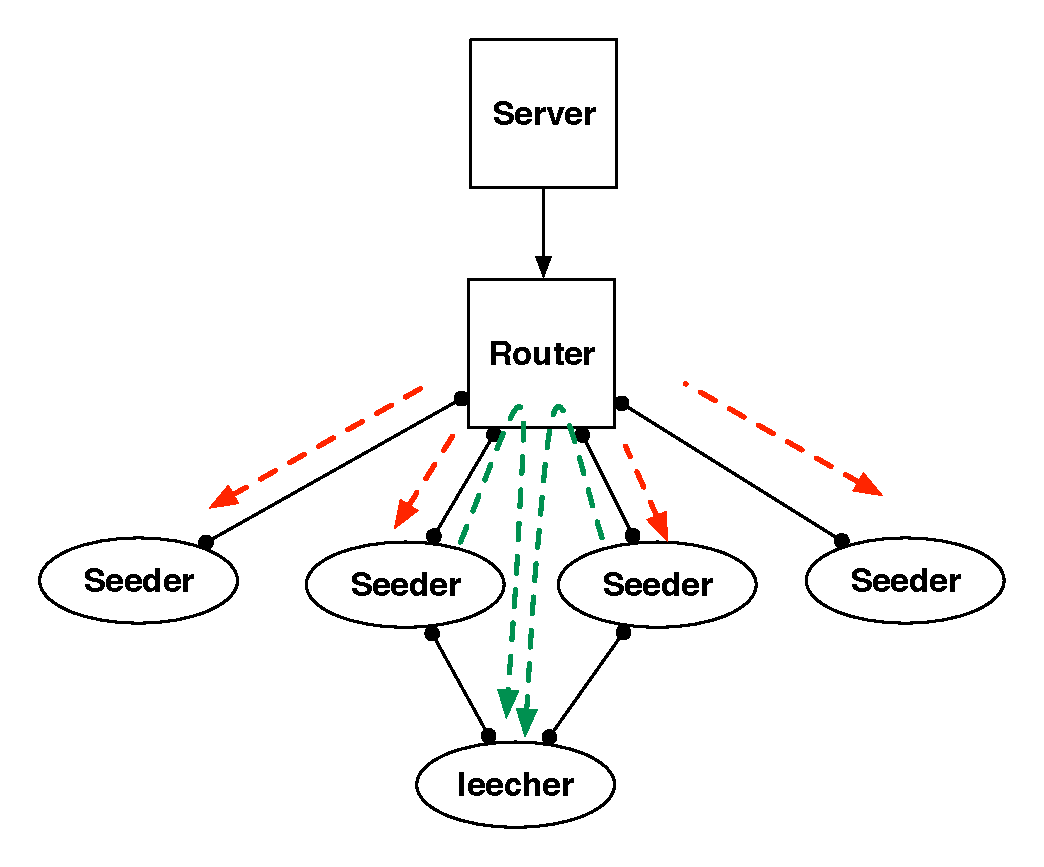
\includegraphics[scale=0.6]{graphs/topology.eps}
\end{center}
\caption{Dummy network}
\label{fig:dummy}
\vspace{-2mm}
\end{figure} 

\begin{table}[thb]
\caption{Numerical Simulation Parameters.}
\label{tab:simparameters}
\hbox to\hsize{\hfil
\begin{tabular}{l|l}\hline\hline
Symbol & Value\\\hline
$\delta_s$ & $5.2 . 10^{-8}$ (J/b)\\
$\delta_r$ & $8.0 . 10^{-9}$ (J/b)\\
$\delta_p$ & $16 . 10^-9$ (J/b)\\
$E_{r-baseline}$ & $750$ watt \\
$E_{s-baseline}$ & $290$ watt \\
$E_{p-baseline}$ & $13.5$ watt \\
%%$B$ & $500$MB\\
$d_s$ & $1$ \\
$N_{s}^{u}$ & $[0.25,0.5,0.75,1]$ Mbps \\
$N$ & $[100,..,1000]$ \\
$T$ & $[20,25]$ correspond to COP value $[3.194,4.728]$\\\hline
\end{tabular}\hfil}
\end{table}

\begin{figure*}[ht]
\centering
\begin{minipage}[b]{0.3\linewidth}
	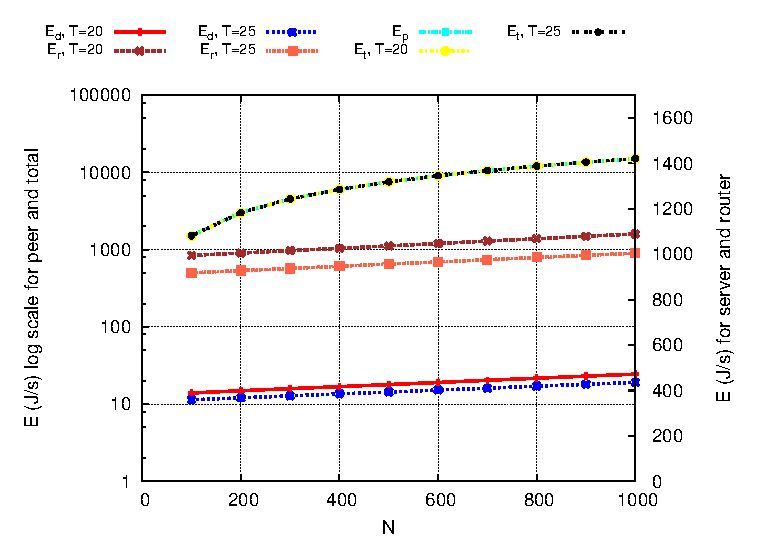
\includegraphics[scale=0.5]{graphs/cdn.eps}
	\caption{CDN.}
	\label{fig:4-0}
\end{minipage}
\hfill
\begin{minipage}[b]{0.3\linewidth}
	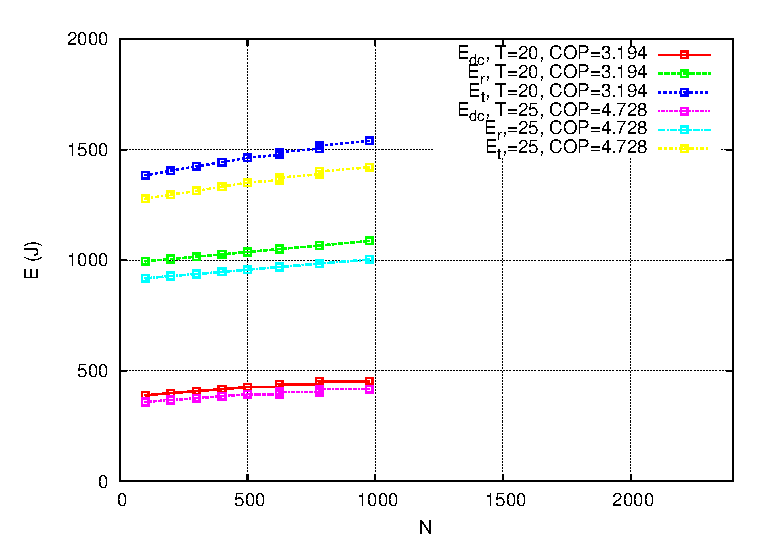
\includegraphics[scale=0.5]{graphs/cdnp2p-1.eps}
	\caption{CDN-P2P $\rho=0.25$.}
	\label{fig:4-1}
\end{minipage}
\hfill
\begin{minipage}[b]{0.3\linewidth}
	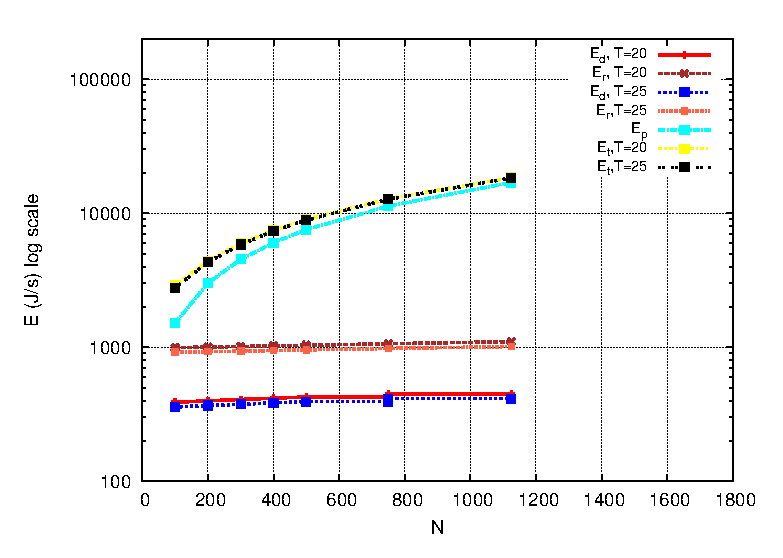
\includegraphics[scale=0.5]{graphs/cdnp2p-2.eps}
	\caption{CDN-P2P $\rho=0.5$.}
	\label{fig:4-2}
\end{minipage}
\hfill
\begin{minipage}[b]{0.35\linewidth}
	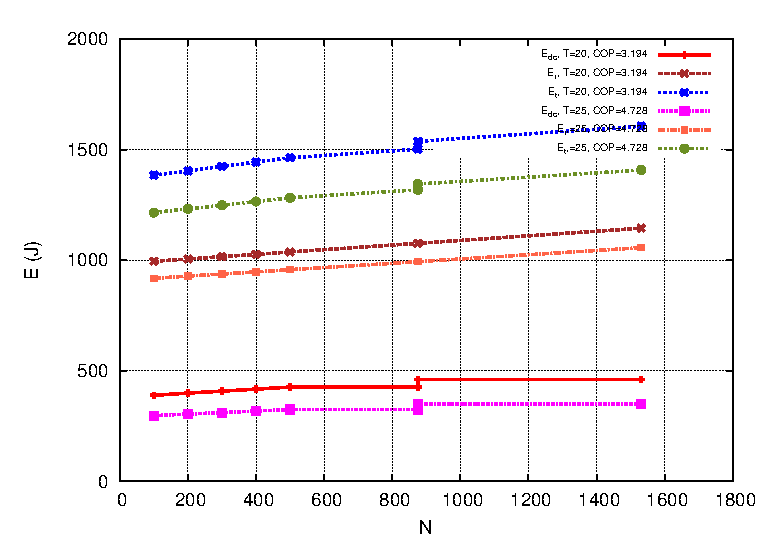
\includegraphics[scale=0.5]{graphs/cdnp2p-3.eps}
	\caption{CDN-P2P $\rho=0.75$.}
	\label{fig:4-3}
\end{minipage}
\hfill
\begin{minipage}[b]{0.35\linewidth}
	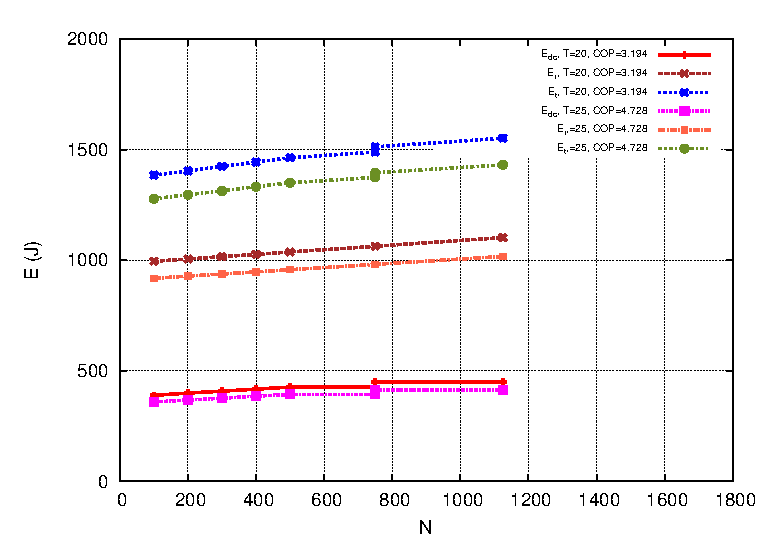
\includegraphics[scale=0.5]{graphs/cdnp2p-4.eps}
	\caption{CDN-P2P $\rho=1$.}
	\label{fig:4-4}
\end{minipage}
%\caption{main}
\label{fig:main}
\end{figure*}


Figure \ref{fig:4-0} shows energy usage for CDN server, router, total energy consumption for CDN scenario (without peer assisted).
We plot energy consumption for CDN server, router, clients, and total energy for every $T$ or $COP$ coefficient value.
In CDN only scenario, the energy consumption is increase as number of client increase.  
This is natural because increasing of clients imply to increasing of traffic from CDN server through router to clients.
The effect of different $T$ to total energy is small.  


\begin{figure*}[ht!]
\centering
\begin{minipage}[b]{0.4\linewidth}
	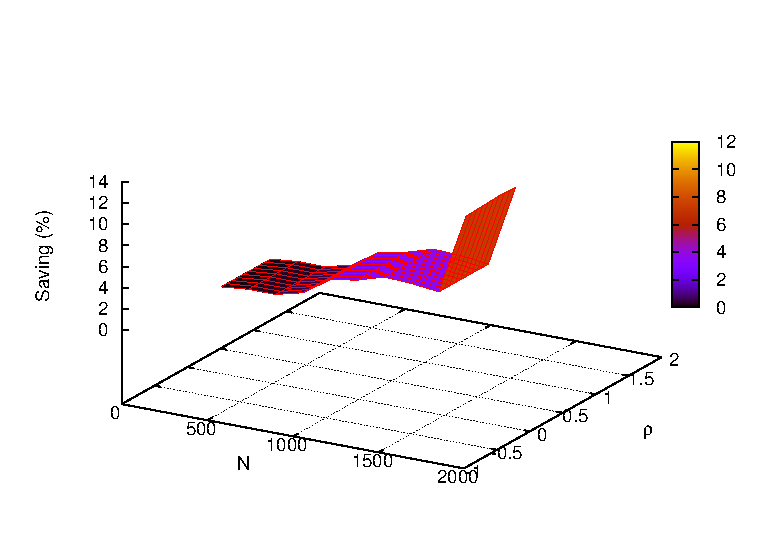
\includegraphics[scale=0.5]{graphs/diff3dimension.eps}
	\caption{Different power consumption between CDN and CDN-P2P for CDN server component with $\rho=0.25,0.5,0.75,1$.}
	\label{fig:diff1}
\end{minipage}
\hfill
\begin{minipage}[b]{0.4\linewidth}
	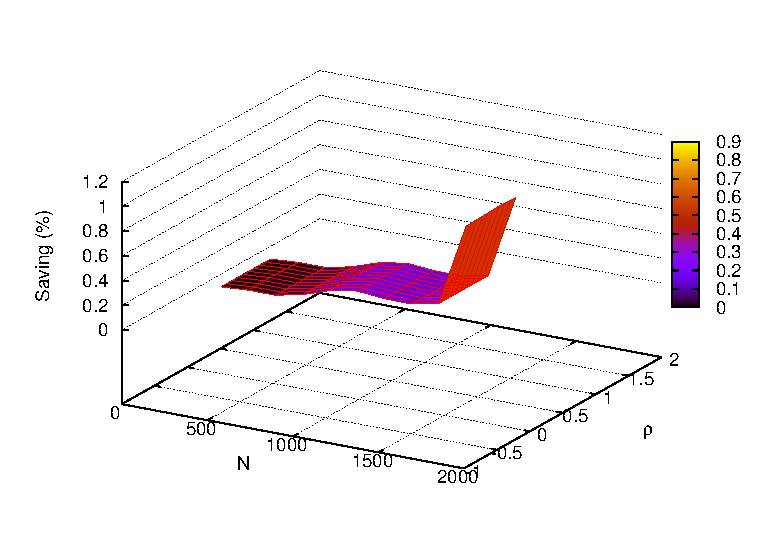
\includegraphics[scale=0.5]{graphs/diff3dimension2.eps}
	\caption{Different power consumption between CDN and CDN-P2P for total system with $\rho=0.25,0.5,0.75,1$.}
	\label{fig:diff2}
\end{minipage}
\label{fig:maindiff}
\end{figure*}



\begin{figure*}[ht!]
\centering
\begin{minipage}[b]{0.4\linewidth}
	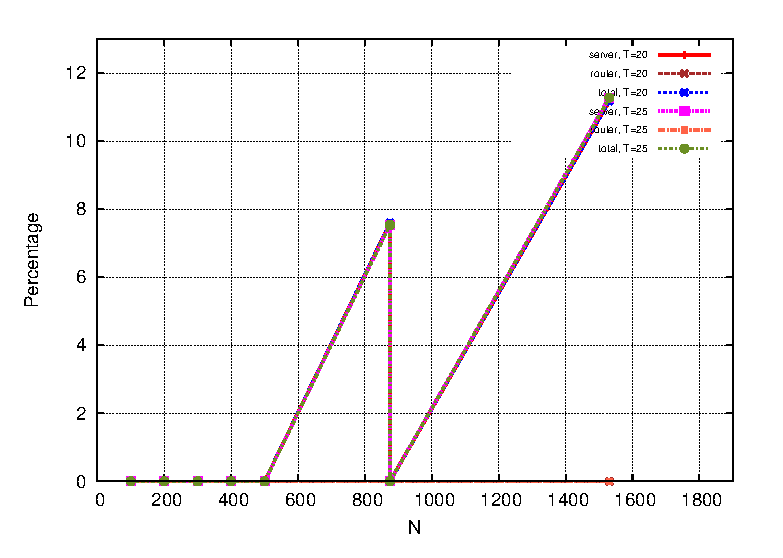
\includegraphics[scale=0.5]{graphs/diff-3.eps}
	\caption{Different power consumption between CDN and CDN-P2P for CDN server component with $\rho=0.75$.}
	\label{fig:diffs1}
\end{minipage}
\hfill
\begin{minipage}[b]{0.4\linewidth}
	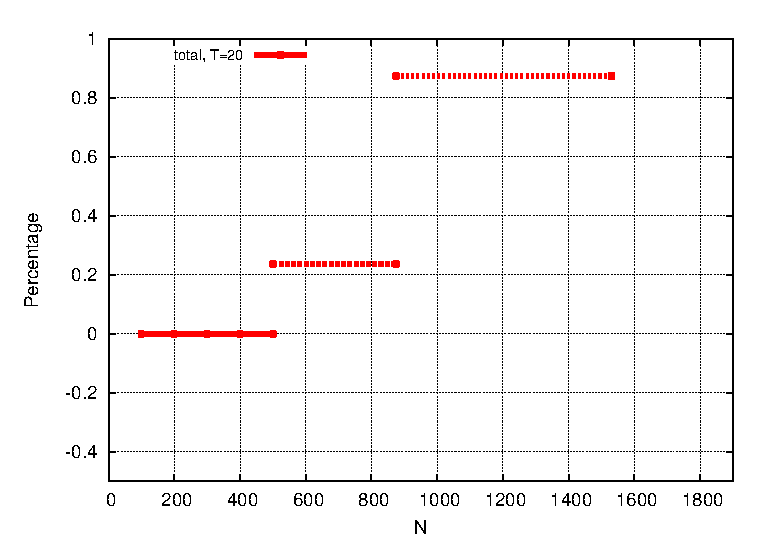
\includegraphics[scale=0.5]{graphs/diff-3-total.eps}
	\caption{Different power consumption between CDN and CDN-P2P for total system with $\rho=0.75$.}
	\label{fig:diffs2}
\end{minipage}
\label{fig:maindiff2}
\end{figure*}



Figure \ref{fig:4-1} shows energy consumption for CDN, router, and total energy consumption for CDN-P2P scenario.
We use upload rate of seeders to leechers $\rho=0.25$.
We assume that CDN server always utilize under $50\%$.
For CDN server energy $E_d$, the usage of energy increase until number of seeders $n_s=500$.
On $n_s=500$ the CDN server right on $50\%$ utilization.
When CDN server on $50\%$ utilization, maximum number of seeders are $n_s=500$ and number of leechers can be served by seeders is $125$ peers.  
Therefore in this situation, CDN server can save energy, because with just $50\%$ utilization, additional $125$ peers can be served from seeders.  
Next, to be able to server more peers, we allow CDN server to increase the utilization to $62.5\%$.
With $62.5\%$ utilization, $625$ peers are served by CDN server. 
Number of leechers can be supported by seeders are $156$ peers.
In this situation CDN server can save energy, because with $62.5\%$ utilization, number additional $156$ peers can be served from seeders.  
In router case, we do not see router can get energy saving because number of traffic increase as increasing number of peers. 
For example, when CDN server on $50\%$ utilization, maximum number seeders are $n_s=500$ and number of leechers can be served by seeders is $125$ peers.
Traffic traverse through router is $500$Mbps plus additional $125$Mbps. 
We get $125$Mbps from $500$ multiply to upload rate of seeders $0.25$Mbps
Different air temperature supply, make different power consumption.  
With $T=25$ or $COP=4.728$, we can see the power consumption for all components lower than $T=20$ or $COP=3.194$.
That's because energy needed to supply air cooling with temperature $T=25$ is less than  energy needed to supply air cooling with temperature $T=20$.


Next, Figure \ref{fig:4-2} reports energy consumption for CDN, router, and total energy consumption for CDN-P2P scenario.
We use upload rate of seeders to leechers $\rho=0.5$.
We assume that CDN server utilization under $50\%$.
For CDN server energy, the usage of energy increase until number of seeders $n_s=500$.
On $n_s=500$ the CDN server right on $50\%$ utilization.
When CDN server on $50\%$ utilization, maximum number of seeders are $n_s=500$ and number of leechers can be served by seeders are $250$ peers.
In this point, CDN server can save energy, because with just $50\%$ utilization, additional $250$ peers are served from seeders. 
In order to allow more peers, then CDN server must allow to increase its utilization from $50\%$ to $75\%$.
With CDN server utilization $75\%$, with number of seeders $n_s=750$ can also serve additional $n_l=325$ leechers.
On the other hand, energy consumption of router increasing with the increasing number of peers because router needs to accommodate traffic from all peers. 

Figure \ref{fig:4-3} presents energy consumption for CDN, router, and total energy consumption for CDN-P2P scenario.  
We use upload rate of seeders to leechers $\rho=0.75$.
We assume that CDN server utilization under $50\%$.
The result almost same with previous. 
CDN server energy increase until number of seeders $n_s=500$.
When CDN server hit $50\%$ utilization, maximum number of seeders are $n_s=500$ and number of leechers can be served by seeders are $325$ peers. 
Therefore with same energy level on $50\%$ utilization the system can server additional $325$ peers. 
Again, router energy consumption is increasing. 

Figure \ref{fig:4-4} shows energy consumption for CDN, router, and total energy consumption for CDN-P2P scenario.  
We use upload rate of seeders to leechers $\rho=1$.
We assume that CDN server utilization under $50\%$.
The result almost same with previous. 
CDN server energy increase until number of seeders $n_s=500$.
When CDN server hit $50\%$ utilization, maximum number of seeders are $n_s=500$ and number of leechers can be served by seeders are $500$ peers. 
Therefore with same energy consumption level on $50\%$ utilization the system can serve additional $500$ peers. 
Once again, router energy consumption is increasing. 


%\begin{figure*}[ht!]
%\centering
%\begin{minipage}[b]{0.3\linewidth}
%	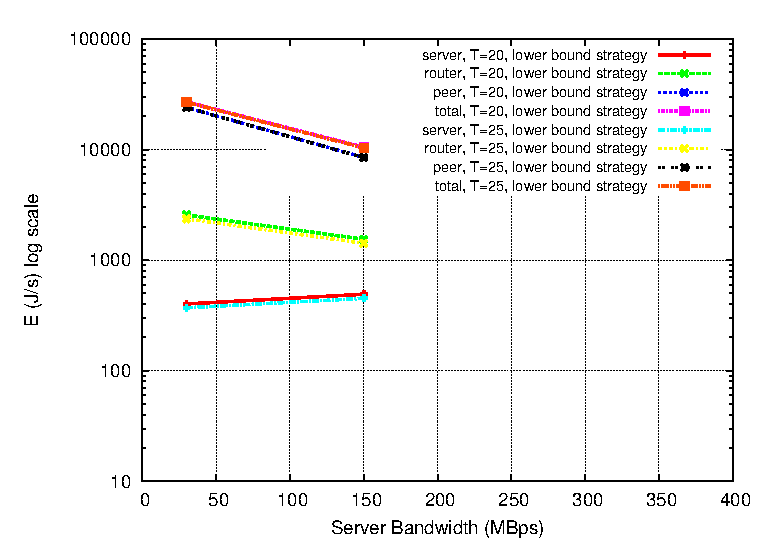
\includegraphics[scale=0.45]{graphs/strategy1.eps}
%	\caption{Power consumption of CDN server, router, and peers in lower bound strategy.}
%	\label{fig:stg1}
%\end{minipage}
%\hfill
%\centering
%\begin{minipage}[b]{0.3\linewidth}
%	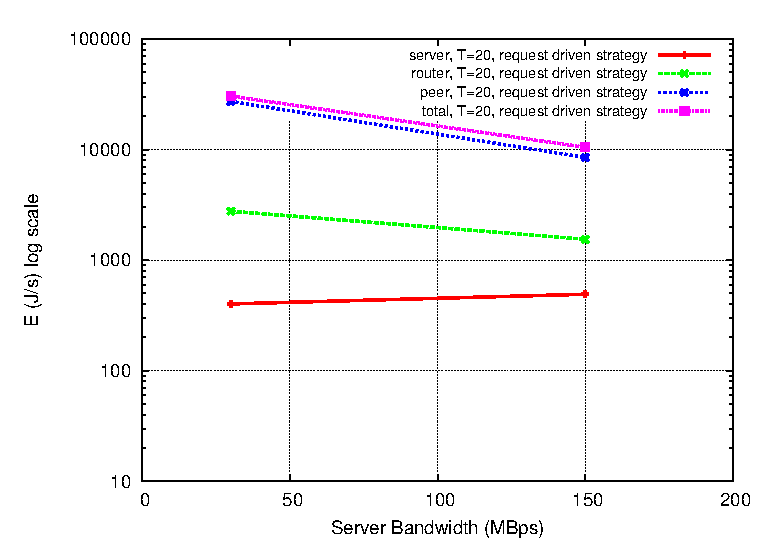
\includegraphics[scale=0.45]{graphs/strategy2.eps}
%	\caption{Power consumption of CDN server, router, and peers in request driven strategy.}
%	\label{fig:stg2}
%\end{minipage}
%\hfill
%\centering
%\begin{minipage}[b]{0.3\linewidth}
%	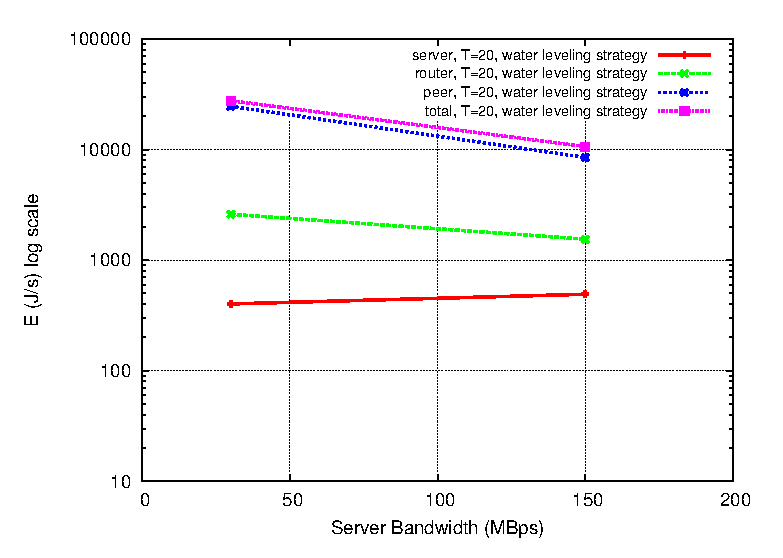
\includegraphics[scale=0.45]{graphs/strategy3.eps}
%	\caption{Power consumption of CDN server, router, and peers, in water leveling strategy.}
%	\label{fig:stg3}
%\end{minipage}
%\caption{main}
%\label{fig:storage}
%\end{figure*}


Figure \ref{fig:diff1} shows percentage difference of energy consumption between CDN and CDN-P2P for CDN server component with $\rho=[0.25,0.5,0.75,1]$.
The power saving that CDN server get is from $3.8\%$ to $11\%$.
More clear figure is shown in fig.\ref{fig:diffs1} that we sliced for $\rho=0.75$ from fig.\ref{fig:diff1}. 
CDN server can save energy because the utilization of CDN server is same when the system has number of peers increasing from $500$ to $875$.
Same situation is also happen when number of peers increasing from $875$ to $1531$.  
The saving is up to $11\%$ 

Figure \ref{fig:diff2} shows percentage difference of energy consumption between CDN and CDN-P2P for total system with $\rho=[0.25,0.5,0.75,1]$.
The power saving that total system get is from $0.2\%$ to $0.9\%$.
Figure \ref{fig:diffs2} reports percentage difference of energy consumption between CDN and CDN-P2P for total system with $\rho=0.75$.
While CDN server part can save more energy, due to peers high energy consumption then total energy saving in the system that we can get is small, from $0.2\%$ to $0.9\%$.
For fig.\ref{fig:diff1}, \ref{fig:diff2}, \ref{fig:diffs1}, and \ref{fig:diffs2}, we only show graph for $T=20$ since the difference with $T=25$ is very small as shown in fig.\ref{fig:4-1} until fig.\ref{fig:4-4}.

\begin{figure*}[ht]
\centering
\begin{minipage}[b]{0.3\linewidth}
	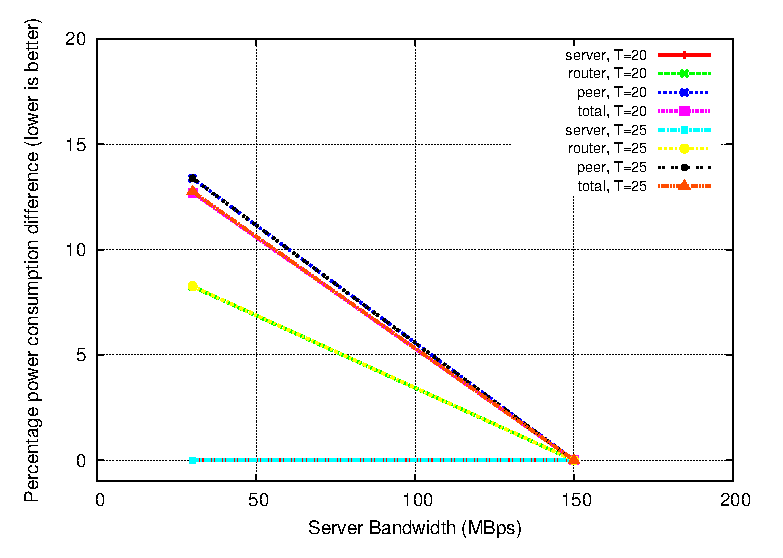
\includegraphics[scale=0.4]{graphs/diff-2to1.eps}
	\caption{Power consumption difference between request driven strategy and lower bound strategy.}
	\label{fig:diff2to1}
\end{minipage}
\hfill
\centering
\begin{minipage}[b]{0.3\linewidth}
	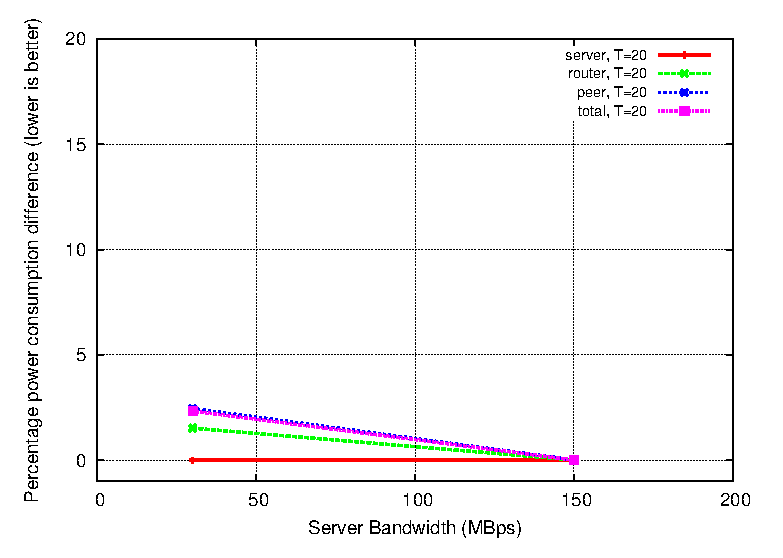
\includegraphics[scale=0.4]{graphs/diff-3to1.eps}
	\caption{Power consumption difference between water leveling strategy and lower bound strategy.}
	\label{fig:diff3to1}
\end{minipage}
\hfill
\begin{minipage}[b]{0.3\linewidth}
	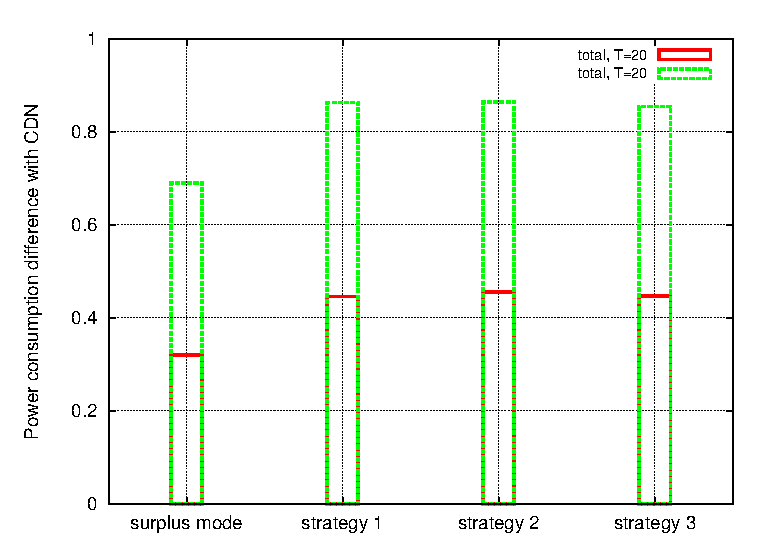
\includegraphics[scale=0.4]{graphs/diff-cdn.eps}
	\caption{Total power consumption difference between CDN architecture, surplus mode, lower bound strategy, request driven strategy, and water leveling strategy.}
	\label{fig:difftocdn}
\end{minipage}
%\caption{main}
\label{fig:diffstrategy}
\end{figure*}

\begin{figure*}[ht]
\centering
\begin{minipage}[b]{0.3\linewidth}
	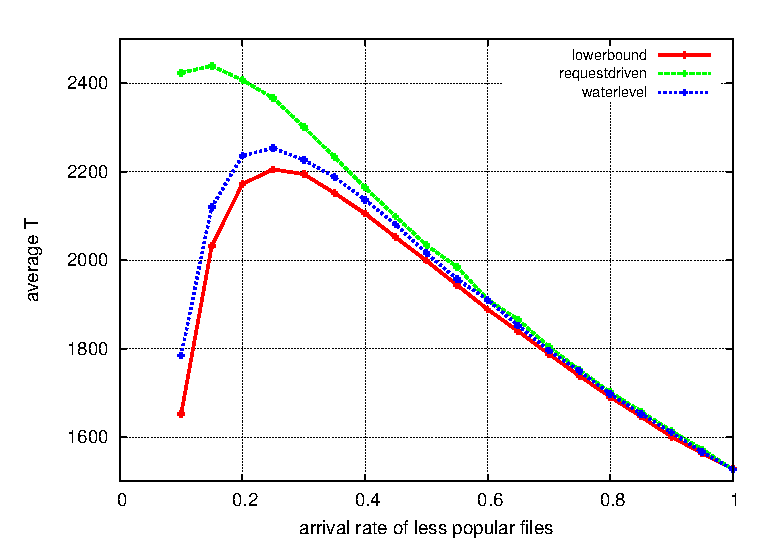
\includegraphics[scale=0.4]{graphs/pop.eps}
	\caption{Comparison of average downloading time under different server bandwidth allocation strategies when the peer arrival rate of less popular files varies.}
	\label{fig:popsimulation}
\end{minipage}
\hfill
\centering
\begin{minipage}[b]{0.3\linewidth}
	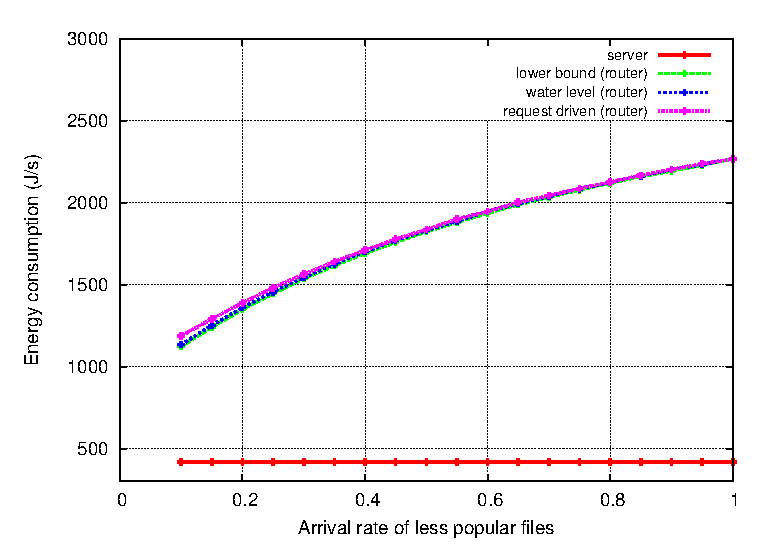
\includegraphics[scale=0.4]{graphs/componentconsumption.eps}
	\caption{Power consumption for server and router under different server bandwidth allocation strategies when the peer arrival rate of less popular files varies. Server bandwidth $S=50$MBps.}
	\label{fig:componentpop}
\end{minipage}
\hfill
\centering
\begin{minipage}[b]{0.3\linewidth}
	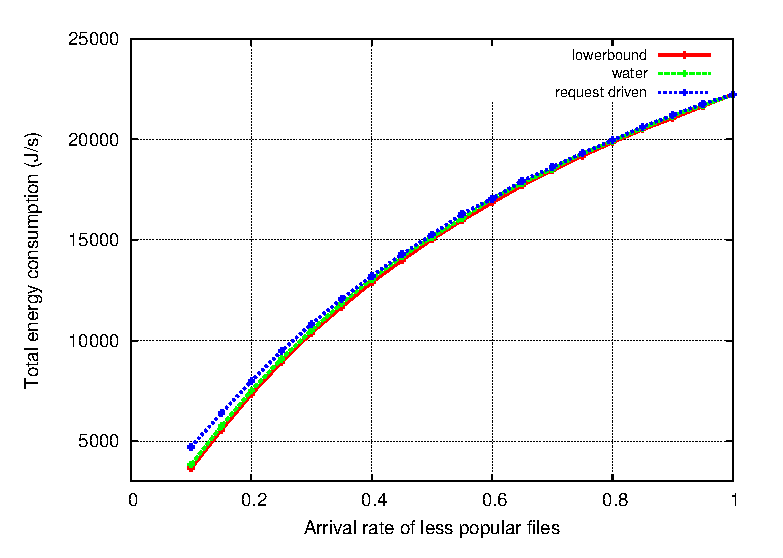
\includegraphics[scale=0.4]{graphs/totalconsumption.eps}
	\caption{Total power consumption under different server bandwidth allocation strategies when the peer arrival rate of less popular files varies. Server bandwidth $S=50$MBps.}
	\label{fig:totalpop}
\end{minipage}
\label{fig:popularity}
\end{figure*}


\subsection{Online Storage}

In peer-assisted online storage, user contribute their upload bandwidth to redistribute of a file that they are downloading or that they have cached locally.
We follow peer-assisted online storage model in \cite{Sun:2009:POS:1542245.1542249} as basis of our work. 
In peer-assisted online storage, users can browse a catalog of available files and asynchronously issue request to download a given file, which are ideally immediately satisfied by the system.
In order to reduce startup latency, first block of file must be downloaded from server \cite{5199550}.
In peer-assisted online storage, users interested to a specific file can retrieve it from servers (CDN) and from users storing copy of it in their computer or dedicated set top boxes/home gateway remotely.  
Peer-assisted online storage model in \cite{Sun:2009:POS:1542245.1542249}, the arrival process of request for considered file follow Poisson process, it takes into account multiple files of different popularity and server bandwidth provisioning.
The model also assume that no peers would abort the download and no peers would stay in the system after finishing downloading the file.
There are three server bandwidth allocation strategies in \cite{Sun:2009:POS:1542245.1542249} which are: (1) lower bound, (2) request driven strategy, and (3) water leveling strategy.
For detail, we refer the readers to \cite{Sun:2009:POS:1542245.1542249,5199550,5061997}.
All numerical simulation parameters that we used in this section same as \cite{Sun:2009:POS:1542245.1542249}.

%Figure \ref{fig:stg1} reports power consumption for lower bound strategy for CDN server, router, and peers, for server bandwidth $S=30$MBps and $S=150$MBps.
%For $S=30$MBps correspond to number of peers $N=1874$ and $S=150$MBps correspond to $N=660$ peers.

%Figure \ref{fig:stg2} reports power consumption for request driven strategy for CDN server, router, and peers, for server bandwidth $S=30$MBps and $S=150$MBps.
%For $S=30$MBps correspond to number of peers $N=2125$ and $S=150$MBps correspond to $N=660$ peers.
%Interestingly, with same $S=30$ compare to lower bound strategy, request driven strategy has more peers. 

%Figure \ref{fig:stg3} reports power consumption for water leveling strategy for CDN server, router, and peers, for server bandwidth $S=30$MBps and $S=150$MBps.
%For $S=30$MBps correspond to number of peers $N=1920$ and $S=150$MBps correspond to $N=660$ peers.
%Compare to lower bound strategy, more number of peers exist in water leveling strategy but less than number of peers in request driven strategy. 

When $S=150$ all of strategies are in server bandwidth surplus mode thus number of peers in the systems are same, while in $S=30$ all of strategies are server bandwidth deficit mode thus number of peers in $S=30$ bigger than number of peers on $S=150$ and number of peers in $S=30$ is also different for every strategies. 
In request driven strategy, server bandwidth is equally divided across all the peers. 
Popular files with more peers involved hence occupy more server bandwidth. 
This behavior explained why more peers exist in request driven strategy.
In water leveling strategy, server bandwidth is equally divided across all the files.  
Fewer peers are involved in less popular files, each of these peers can obtain more server bandwidth.  
This explains less peers compare to request driven but more peers compare to lower bound.

Request driven strategy totally consume around $12\%$ more energy compare to lower bound strategy fig.\ref{fig:diff2to1}, while water level strategy totally consume around $2.3\%$ more energy compare to lower bound strategy fig.\ref{fig:diff3to1}.
Compare to CDN architecture, peer-assisted CDN online storage can save total energy around $0.45\%$ if we add cooling overhead $T=20$ and around $0.8\%$ if we have cooling overhead $T=25$ fig.\ref{fig:difftocdn}.
%Generally, increasing server bandwidth will decrease number of peers thus increasing CDN server energy consumption and decreasing router energy consumption. 
%Total energy consumption in every strategies depend on number peers.  

File popularity has strong correlation with downloading performance. 
We examine popularity by varying the peer arrival rate of less popular files.
Specifically we linearly increase file popularity from $0.1$ to $1$ and we choose server bandwidth $S=50$MBps which is quite constraint and similar to FS2You case.
As shown in fig.\ref{fig:popsimulation} when file popularity increases, downloading performance decrease first and increases again as files become more popular.
When file popularity is low there are fewer peers downloading the file and hence each of them can obtain relatively more sever bandwidth.
When file popularity is high peers can enjoy high file sharing effectiveness and hence high average downloading rates.
Semi popular files get the worst downloading performance in the system as difficulty in both file sharing among peers and requesting bandwidth from server.
In request driven strategy, we do not find such as U-shaped curve due to server bandwidth strategy that is equally divided across all peers and not affected by file popularity.

Figure \ref{fig:totalpop} shows total energy of system as function from file popularity.  
More popular file imply having more peers in the system thus increases total energy.  
While CDN server energy consumption is constant, router energy consumption is increases fig.\ref{fig:componentpop}. 



\section{Related Work} 

Content Distribution Networks with peer assist have been successfully deployed on the Internet, such as Akamai \cite{Huang:2008:UHC:1496046.1496064} and LiveSky \cite{Yin:2010:LEC:1823746.1823750}.  
The authors of \cite{Huang:2008:UHC:1496046.1496064} conclude from two real world traces that hybrid CDN-P2P can significantly reduce the cost of content distribution and can scale to cope with the exponential growth of Internet video content.  
Yin et al. \cite{Yin:2010:LEC:1823746.1823750} described LiveSkye as commercial operation of a peer-assisted CDN in China.  
LiveSky solved several challenges in the system design, such as dynamic resource scaling of P2P, low startup latency, ease of P2P integration with the existing CDN infrastructure, and network friendliness and upload fairness in the P2P operation.  
Measurement from LiveSky showed that LiveSky can save bandwidth around 40\% \cite{Yin:2010:LEC:1823746.1823750}.
The author in \cite{Huang:2007:IVP:1282427.1282396} and \cite{huang2007peer} proposed mechanisms to minimize CDN server bandwidth to make the content distribution cheap.
They designed different peer prefetching policies of video on demand system in surplus mode while ensuring user quality of experience.
A similar analysis has been done in \cite{xu2006analysis} for live video streaming system where the authors proposed different limited peer contribution policies to reduce CDN bandwidth requirement and eventually off the distribution process from CDN to P2P system. 
An ISP friendly rate allocation schemes for a hybrid CDN-P2P video on demand system in \cite{Wang:2008:IRA:1459359.1459397}. 
These technique try to minimize CDN server bandwidth while reducing ISP unfriendly traffic and maximizing peer prefetching.
Load on CDN server has been shown to be reduced using this approach while reducing cross ISP traffic.
Above studies were performed for video on demand or live video streaming.
While video is the most popular content, the systems can be also for other type contents.
Moreover while content based services are growing, energy consumption of a content distribution system has not been analyzed.

Related to CDN and energy usage, in a seminal work \cite{qureshi2009cutting}, the authors show that if costs are based on electricity usage and if the power prices vary in real-time, global load balancing decision can be made such that users are routed to locations with the cheapest power without significantly impacting user performance or bandwidth cost.  
In \cite{Palasamudram:2012:UBR:2391229.2391240}, the author proposed utilizing batteries for CDN for reducing total supplied power and total power costs.
The authors in \cite{Palasamudram:2012:UBR:2391229.2391240} also proposed battery provisioning algorithms based on workload of CDN server. 
The result shows that batteries can provide up to 14\% power savings.

The idea that utilize ISP controlled home gateway to provide computing and storage services and adopts managed peer-to-peer model is presented in \cite{valancius2009greening}. 
Valancius et al. \cite{valancius2009greening} show that distributing computing platform in NaDa (Nano Data Center) save at least 20-30\% energy compare to traditional data centers.
The saving in NaDa comes from underutilizing home gateway, avoidance of cooling costs, and the reduction of network energy consumption as a result of demand and service co-localization.

The comparison between CDN architecture and peer-to-peer architecture are discussed in \cite{baliga2007energy} and \cite{feldmann2010energy}.
Both authors in \cite{baliga2007energy} and \cite{feldmann2010energy} agree that CDN architecture is more energy saving compare to peer-to-peer architecture. 
Another interesting study of energy efficient in content delivery architectures is presented by Guan et al. \cite{5963557}.
by Guan et al. \cite{5963557} comparing energy efficient of CDN architecture and CCN architecture.
The authors in \cite{5963557} conclude that CCN is more energy efficient in delivering popular content while the approach with optical bypass is more energy efficient in delivering infrequent accessed content.

To the best of our knowledge, the study of energy in that considering peer-to-peer in CDN architecture is presented in \cite{6524219}.
Mandal et al. \cite{6524219} mentioned that hybrid CDN-P2P systems can reduce a significant amount energy in the optical core network around 20-40\% less energy.  
The authors only considered energy consumption of hardware especially optical devices and does not include overhead inside data center, CDN server energy comsumption, and consumed power by peers.
Our work is quite different, we take number of peers and add overhead of data center which is power of cooling cause by temperature of hardware for different purpose: live streaming and online storage.

\section{Conclusion and Future Work}\label{conclusion}

In this paper, we have introduced the comparison of energy consumption between the peer-assisted CDN architecture and CDN architecture for live streaming and video on demand service.
Integrating peer to peer capability to assist the existing CDN has a potential to save energy consumption.
In this study, we show that event without explicitly considering energy consumption while assigning content, the peer assisted CDN can save energy consumption.
Although the energy savings depend on number of request (number of clients), number of router and its configuration, for total system energy saving is around $0.5$ to $1.2$.
If we break per component, the CDN server is the part that can be pushed to save energy up to $11\%$ and can be more if new generation of power proportional server is used \cite{Krioukov:2011:NDI:1925861.1925878}.
We agree with \cite{4509688}, Router component in the other side is quite difficult to optimize for energy saving, because different chassis size, different network interface type slot, and different configuration can lead to different energy consumption.
Several areas that we have been identified for future work are: more correlation analysis of time period to peer energy usage pattern in live streaming, continued characterization of different peer energy usage based on flash memory storage, and comparing energy model with different file popularity models.


\section*{Acknowledgements}
We thank A,B,C, and D

\bibliographystyle{IEEEtran}% bib style
\bibliography{journal}% your bib database



%\begin{biography}
%
%\profile{Mohamad Dikshie Fauzie}{was born in 1976.\
%He received a bachelors degree and a master's degree from Institute of Technology Bandung, Indonesia.\
%He is currently a Ph.D candidate at Keio University's Shonan Fujisawa Campus.}
%
%\profile{Achmad Husni Thamrin}{is Assistant Professor at Keio University.\ 
%He is a graduate of Keio University, Graduate School of Media and Governance (Ph.D 2005, MMG, 2002).\
%His research interests include multicast, Internet over broadcast media, and peer-to-peer networks.} 
%
%\profile{Jun Murai}{was born in March 1955 in Tokyo.\
%Graduated Keio University in 1979, Department of Mathematics, Faculty of Science and Technology.\
%He received his M.S. for Computer Science from Keio University in 1981,
%and received his Ph.D. in Computer Science, Keio University in 1987.\ 
%He specializes in computer science, computer network, and computer 
%communication. He is currently Dean of the Faculty of Environment and Information Studies, Keio University since October 2009.\
%Former Vice-President of Keio University from May 2005 to May 2009.\ 
%He was an Executive Director of the Keio Research Institute at SFC, Keio University from 1999 to 2005.}
%
%\end{biography}

\end{document}
